\documentclass{article}
\usepackage{graphicx}
\usepackage{tocloft} 
\usepackage{glossaries}
\usepackage{lipsum}
\usepackage{geometry}
\usepackage{fancyhdr} 
\usepackage{amsmath}
\usepackage{biblatex}  

\addbibresource{../common/references.bib}  

\geometry{a4paper, margin= 1in}

\makeglossaries
\loadglsentries{../common/glossary}

\title{Software Design Document (SDD)}
\author{Group 1 }
\date{December 1 2024}

\begin{document}
\maketitle  
\pagebreak

\tableofcontents
\pagebreak

\section*{Version History}
\begin{longtable}{|c|c|p{10cm}|}
\hline
\textbf{Version} & \textbf{Date} & \textbf{Description} \\ \hline
3.0 & December 1 2024 & Finished Section 2.1 \\ \hline
2.0 &November 20, 2024 & Added glosary and references \\ \hline
1.0 & November 20 2024 & Began document and laid out the foundation \\ \hline
\end{longtable}
\pagebreak


\includegraphics[width=0.3\linewidth]{../logo/csula.png} 

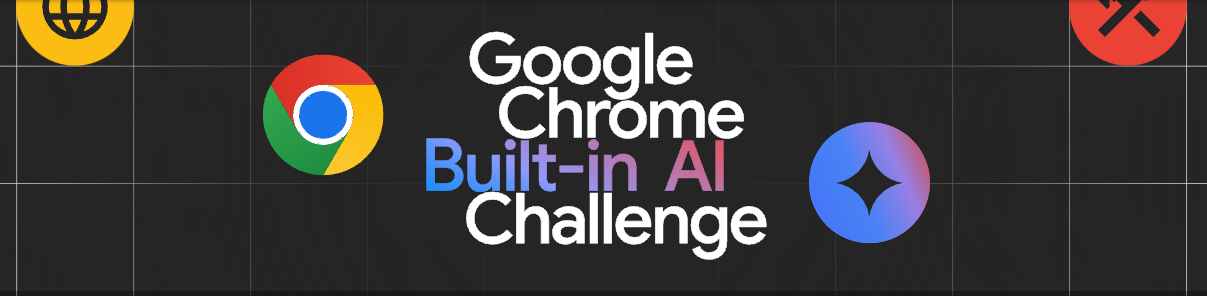
\includegraphics[width=0.3\linewidth]{../logo/chromeai.png} 
\section{Introduction}

\subsection{Purpose}
Our project is based on a competition from Google to use Chrome's built in \Gls{ai} API's to interact with Gemini Nano or other AI Models in a web app or Chrome browser extension. 

The competition is available at https://googlechromeai.devpost.com/

\subsection{Intended Audience}
Our Project Management system is designed to cater to Project Managers, Software Teams, Technical Stakeholders, and any individual or organization that requires a project management tool and values AI integration for task management. Whether it's automating task descriptions, simplifying project oversight, or improving team collaboration, our system is designed to meet the needs of both small teams and large organizations looking to optimize their project management processes.


\subsection{Overview}
Our web application is a Project Management System similar to TestRails or Jira, using the built in Chrome \Gls{ai} API we will include ai generated descriptions and task creations with voice input. We use the Chrome developer documentation\cite{dev} as main reference for developing a chrome extension.

\section{System Architecture}

\subsection{Workflow}

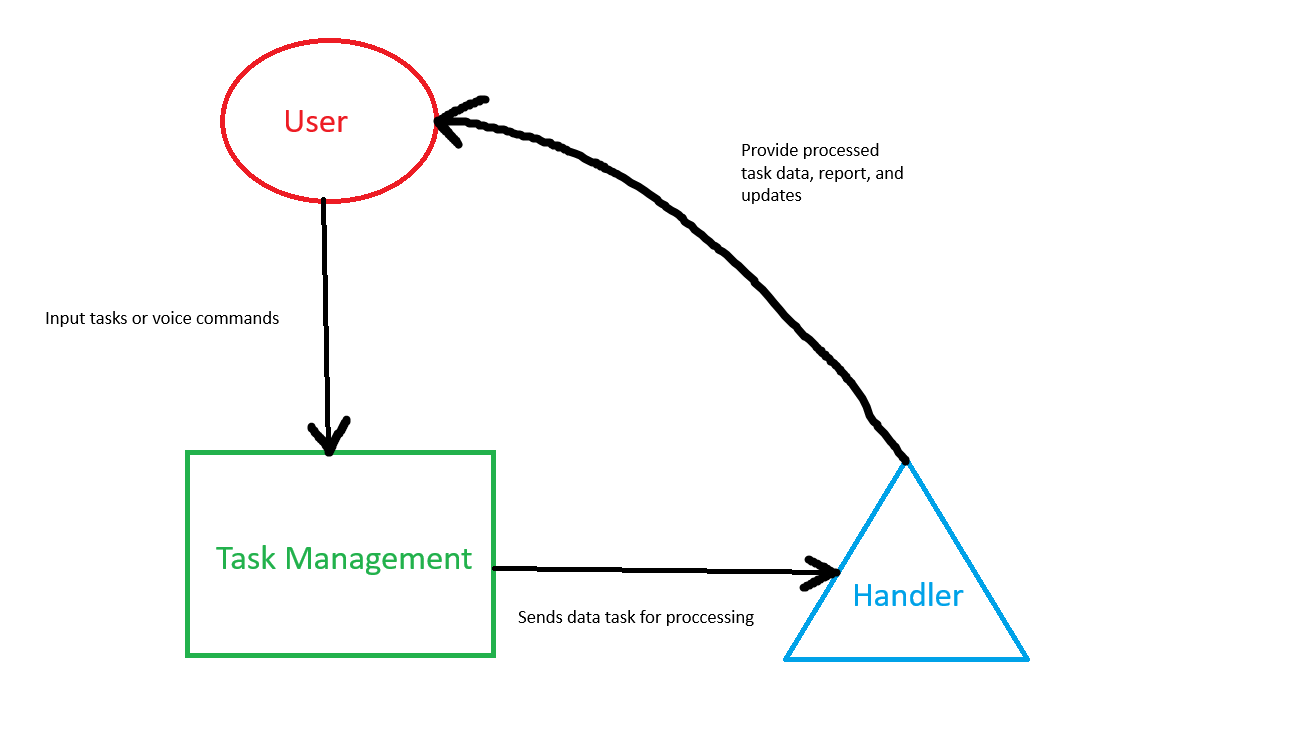
\includegraphics[width=0.9\linewidth]{../logo/workflow.png} 

\begin{itemize}
    \item User: The user interacts with the system through the web interface or Chrome extension. Voice inputs are then captured using the Chrome Speech API for task creation. Commands and inputs are sent to the server for processing.
    \item AI-Driven Task Management: User inputs are analyzed by AI algorithms on the server. AI generates task descriptions and suggestions, which are then sent back to the client-side for user review.
    \item Data Handler: Task and project data are stored and retrieved from a central database. Real-time updates are sent to clients.
    \item Project Update: Updates are processed and visualized on the dashboard in realtime. AI-generated insights and reports are prepared server-side and displayed to user.
\end{itemize}

 
\section{User Interface}

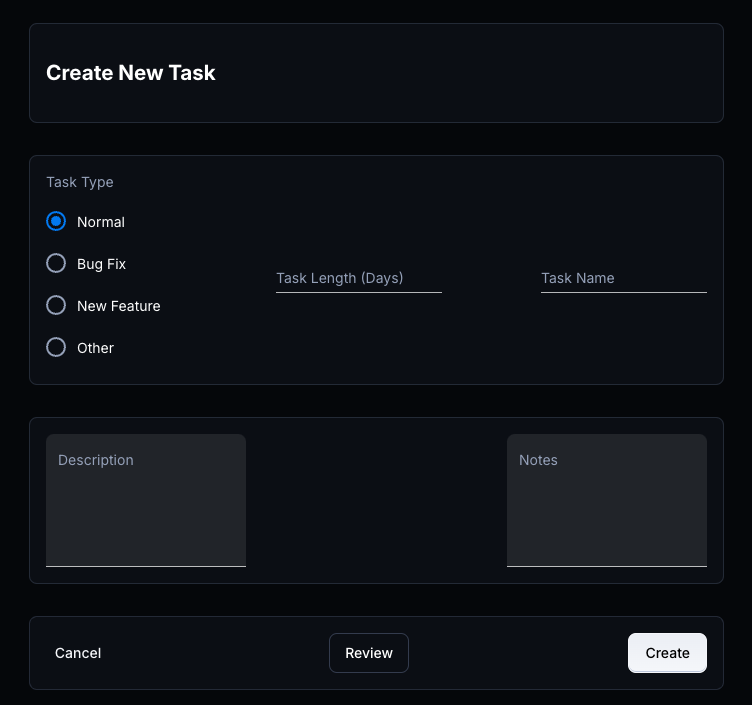
\includegraphics[width=0.9\linewidth]{../logo/mockup.png} 

The Ui is based on Material Ui\cite{mui}, the create new task page is shown above.

\subsection{Database}
The database is a simple \Gls{sql} layout with a userid look table and a main task table. Users can only access tasks that were created by or shared to their userid.


\pagebreak
\printglossaries

% include references.
\printbibliography
\end{document}